% =============================================================================
% Integrantes: Arthur Meneses Neves, Danilo Oliveira Santos, Matheus Gabriel
% Viana Araujo, João Victor Vidal Barbosa, Guilherme Araujo Castro
%
% Síntese: Artigo parcial (Parte 2 / N1) do projeto da disciplina de
% Inteligência Artificial, no template SBC. Descreve o problema (classificar
% o capítulo CID-10 da causa básica de óbito a partir de atributos
% sociodemográficos do SIM, 2000-2026, Brasil), a fundamentação teórica e os
% trabalhos relacionados, a metodologia (divisão estratificada, pesos
% balanceados, prevenção de vazamento de rótulo, F1-macro / recall por classe
% / matriz de confusão), o dataset com sua análise exploratória e preparação,
% os aspectos éticos (LGPD, CEP) e os resultados parciais comparando um
% baseline de classe majoritária, Random Forest e XGBoost. Todos os números
% citados vêm das saídas executadas dos notebooks 01, 02 e 03.
%
% Changelog:
%   2026-09-24 — Matheus Araujo — criação do artigo parcial (SBC)
% =============================================================================

\documentclass[12pt]{article}

\usepackage{sbc-template}
\usepackage{graphicx,url}
\usepackage[utf8]{inputenc}
\usepackage[brazil]{babel}

\sloppy

\title{Classificação da Causa Básica de Óbito pelo Capítulo da CID-10:\\
  uma Comparação entre Random Forest e XGBoost}

\author{Arthur Meneses Neves (RA 10425727), Danilo Oliveira Santos (RA 10410905),\\
  Guilherme Araujo Castro (RA 10427775), João Victor Vidal Barbosa (RA 10410165),\\
  Matheus Gabriel Viana Araujo (RA 10420444)}

%% REVISAR PELO GRUPO: os e-mails institucionais estão pendentes e são
%% preenchidos na Tabela de integrantes, no início da Seção 1.
\address{Faculdade de Computação e Informática --
  Universidade Presbiteriana Mackenzie (UPM)\\
  São Paulo -- SP -- Brasil
  \email{e-mails institucionais: ver Tabela~\ref{tab:integrantes}}
}

\begin{document}

\maketitle

\begin{abstract}
  This paper reports the first-bimester results of an applied AI project that
  classifies the underlying cause of death, aggregated into its ICD-10
  chapter, from five sociodemographic attributes recorded in Brazil's
  Mortality Information System (SIM): age, sex, race/skin colour, schooling
  and state of residence. The study covers Brazil as a whole between 2000 and
  2026 (32,531,918 records after preparation, 19 observed ICD-10 chapters).
  Random Forest and XGBoost, trained with balanced sample weights on a
  stratified 80/20 split, are compared against a majority-class baseline using
  macro-F1, per-class recall and confusion matrices. XGBoost reaches a
  macro-F1 of 0.1406 and Random Forest 0.1329, against 0.0224 for the
  baseline; absolute performance is low, which we interpret as evidence that
  sociodemographic attributes alone carry limited signal about the cause of
  death. We also describe the exploratory analysis, the data preparation,
  the explicit prevention of label leakage and the ethical and legal
  considerations of the approach.
\end{abstract}

\begin{resumo}
  Este artigo relata os resultados do primeiro bimestre de um projeto de IA
  aplicada que classifica a causa básica de óbito, agregada em seu capítulo
  da CID-10, a partir de cinco atributos sociodemográficos registrados no
  Sistema de Informação sobre Mortalidade (SIM): idade, sexo, raça/cor,
  escolaridade e unidade da federação de residência. O recorte é o Brasil
  inteiro entre 2000 e 2026 (32.531.918 registros após a preparação, 19
  capítulos CID-10 observados). Random Forest e XGBoost, treinados com pesos
  de amostra balanceados sobre uma divisão estratificada 80/20, são
  comparados a um baseline de classe majoritária por F1-macro, recall por
  classe e matrizes de confusão. O XGBoost alcança F1-macro de 0,1406 e o
  Random Forest 0,1329, contra 0,0224 do baseline; o desempenho absoluto é
  baixo, o que interpretamos como evidência de que atributos
  sociodemográficos isolados carregam pouco sinal sobre a causa do óbito.
  Descrevemos também a análise exploratória, a preparação dos dados, a
  prevenção explícita de vazamento de rótulo e as considerações éticas e
  legais da abordagem.
\end{resumo}

\section{Introdução}

%% REVISAR PELO GRUPO: preencher a coluna de e-mail institucional de cada
%% integrante na tabela abaixo antes do envio pelo AVA.
\begin{table}[ht]
\centering
\caption{Integrantes do grupo (turma 7º N, Ciência da Computação).}
\label{tab:integrantes}
\begin{tabular}{|l|l|l|}
\hline
\textbf{Integrante} & \textbf{RA} & \textbf{E-mail institucional} \\
\hline
Arthur Meneses Neves         & 10425727 & \texttt{[pendente]} \\
Danilo Oliveira Santos       & 10410905 & \texttt{[pendente]} \\
Guilherme Araujo Castro      & 10427775 & \texttt{[pendente]} \\
João Victor Vidal Barbosa    & 10410165 & \texttt{[pendente]} \\
Matheus Gabriel Viana Araujo & 10420444 & \texttt{[pendente]} \\
\hline
\end{tabular}
\end{table}

\subsection{Contextualização}

O Sistema de Informação sobre Mortalidade (SIM) é o sistema do Ministério da
Saúde que consolida as Declarações de Óbito emitidas no país. Seus microdados
individuais estão disponíveis desde 1996, obtidos do DATASUS e publicados como
dados abertos~\cite{pcdas_sim,sim_dadosgov}. Cada registro traz, além da causa
básica do óbito codificada segundo a Classificação Internacional de Doenças,
10ª revisão (CID-10)~\cite{who_cid10}, atributos sociodemográficos do falecido
e dados de residência e ocorrência.

A CID-10 organiza os milhares de códigos individuais em capítulos, numerados
em algarismos romanos, que agrupam causas afins --- doenças do aparelho
circulatório, neoplasias, causas externas, e assim por diante. Trabalhar no
nível de capítulo, e não no do código completo, transforma um problema de
centenas ou milhares de classes em um problema com poucas dezenas de classes,
tratável com os algoritmos de aprendizado supervisionado vistos na disciplina.

Este projeto trabalha com o recorte \textbf{Brasil, âmbito nacional, período
de 2000 a 2026} (2026 é um ano parcial, pois o arquivo ainda estava em
formação no momento do download). A delimitação inferior em 2000 é técnica: o
SIM usou a CID-9, com códigos puramente numéricos, até 1995, e não há
mapeamento limpo de capítulo entre os dois esquemas de codificação.

\subsection{Justificativa}

Entender como fatores sociodemográficos --- idade, sexo, raça/cor,
escolaridade e localização --- se relacionam à categoria da causa de óbito é
relevante para o planejamento de políticas públicas de saúde: onde alocar
recursos de prevenção, quais grupos priorizar em campanhas e quais padrões
regionais merecem investigação. O tema se alinha diretamente ao Objetivo de
Desenvolvimento Sustentável 3 (Saúde e Bem-Estar), cuja meta 3.4 prevê reduzir
em um terço, até 2030, a mortalidade prematura por doenças não
transmissíveis~\cite{ods3}.

Há também uma justificativa metodológica. O SIM é uma base grande, pública e
heterogênea entre anos, e a própria literatura registra limitações
persistentes na qualidade do preenchimento das declarações de
óbito~\cite{morais2017}. Medir quanto sinal existe apenas nos atributos
sociodemográficos --- e reportar honestamente esse limite --- é um resultado
útil por si só, porque delimita o que se pode e o que não se pode esperar de
modelos construídos sobre esse subconjunto de variáveis.

\subsection{Motivação}

%% REVISAR PELO GRUPO: esta subseção está escrita a partir do contexto
%% objetivo do projeto. Se o grupo quiser acrescentar a motivação pessoal de
%% cada integrante, este é o lugar.
A motivação do grupo para este tema combina três fatores. Primeiro, o
interesse em aplicar as técnicas de aprendizado de máquina da disciplina a um
problema de saúde pública com impacto social claro, e não a um conjunto de
dados sintético ou didático. Segundo, a disponibilidade de uma base pública,
gratuita e de escala real: são 27 arquivos anuais e mais de 32 milhões de
registros, um volume que obriga o grupo a lidar com questões práticas de
engenharia de dados --- formatos que mudam entre anos, memória, tempo de
treino --- que não aparecem em bases pequenas. Terceiro, o fato de a tarefa
ser genuinamente difícil e de desfecho incerto: não sabíamos, ao propor o
projeto, quanto da causa de óbito seria previsível a partir de variáveis
sociodemográficas, e responder a essa pergunta com evidência empírica é mais
instrutivo do que reproduzir um resultado já conhecido.

\subsection{Objetivo}

O objetivo é \textbf{classificar a causa básica de óbito, agregada em seu
capítulo da CID-10}, a partir de atributos sociodemográficos registrados no
SIM. Explicitamente:

\begin{itemize}
  \item \textbf{Variáveis de entrada (atributos):} idade em anos completos
    (numérica), sexo (masculino, feminino), raça/cor autodeclarada (branca,
    preta, amarela, parda, indígena, ignorado), escolaridade (nenhuma, 1 a 3
    anos, 4 a 7 anos, 8 a 11 anos, 12 anos ou mais, ignorado) e unidade da
    federação de residência, derivada do código do município de residência
    (27 categorias). São cinco variáveis.
  \item \textbf{Variável de saída (classes):} o capítulo da CID-10 da causa
    básica, com $k = 19$ classes efetivamente observadas nos dados (capítulos
    I a XVIII e XX; os capítulos XIX e XXI nunca ocorrem como causa básica
    nesta base). A lista completa das classes e sua frequência estão na
    Tabela~\ref{tab:classes}.
  \item \textbf{Período:} 2000 a 2026, sendo 2026 um ano parcial.
  \item \textbf{Região:} Brasil, âmbito nacional, sem recorte por estado ou
    região.
\end{itemize}

Nenhuma variável que descreva a cadeia de causas da própria declaração de
óbito (campos \texttt{LINHAA}--\texttt{LINHAD}, \texttt{CIRCOBITO},
\texttt{CAUSABAS\_O}) é usada como entrada, para evitar vazamento do rótulo;
a Seção~\ref{sec:metodologia} detalha como isso é garantido e verificado em
código.

\subsection{Contribuições esperadas}

\begin{enumerate}
  \item Uma análise exploratória documentada e reprodutível do SIM 2000--2026,
    incluindo as inconsistências de formato entre anos e a evolução do
    não-preenchimento de raça/cor e escolaridade.
  \item Uma função de mapeamento \texttt{CAUSABAS} $\rightarrow$ capítulo
    CID-10 reutilizável, com testes automatizados, e uma rotina única de
    preparação dos dados compartilhada por todos os notebooks.
  \item Uma comparação entre um baseline de classe majoritária, Random Forest
    e XGBoost para essa tarefa, com discussão explícita de desempenho por
    classe, custo computacional, desbalanceamento e limitações.
  \item Uma medida empírica de quanto sinal sobre a causa de óbito existe
    apenas em atributos sociodemográficos, reportada sem superestimação.
\end{enumerate}

\section{Fundamentação Teórica e Trabalhos Relacionados}

\subsection{Conceitos fundamentais}

O problema tratado é de \textbf{classificação supervisionada multiclasse}:
dado um vetor de atributos $x$, atribuir a ele um rótulo $y$ entre $k$
classes mutuamente exclusivas, aprendendo a associação a partir de exemplos
rotulados. Os dois algoritmos comparados pertencem à família dos
\emph{ensembles} de árvores de decisão, hoje o padrão de referência para
dados tabulares.

\textbf{Random Forest}~\cite{breiman2001} treina um conjunto de árvores de
decisão, cada uma sobre uma amostra bootstrap dos dados e com uma seleção
aleatória de atributos em cada nó; a predição final é o voto da maioria. A
aleatorização reduz a correlação entre as árvores, e o erro de generalização
da floresta depende da força das árvores individuais e dessa correlação. É um
método robusto a atributos irrelevantes e de treino naturalmente paralelizável.

\textbf{XGBoost}~\cite{chen2016} implementa \emph{gradient boosting}: as
árvores são construídas em sequência, cada uma ajustada ao erro residual das
anteriores, com regularização explícita da complexidade. O trabalho original
descreve um algoritmo consciente de esparsidade e um esquema aproximado de
busca de pontos de corte por histogramas (\emph{weighted quantile sketch}),
que é justamente o que torna o método viável em bases com dezenas de milhões
de linhas, como a nossa.

Dois conceitos adicionais estruturam a metodologia. O primeiro é o
\textbf{desbalanceamento de classes}: quando uma classe domina a base, a
acurácia deixa de ser informativa, porque um classificador trivial que sempre
prevê a classe majoritária já a maximiza. Por isso adotamos o
\textbf{F1-macro}, que é a média aritmética simples do F1 de cada classe e,
portanto, dá o mesmo peso a um capítulo com 8,8 milhões de registros e a um
com 629, além do recall por classe e da matriz de confusão. O segundo é o
\textbf{vazamento de rótulo} (\emph{label leakage}): a presença, entre os
atributos, de informação que só existe porque o rótulo já é conhecido. Em uma
base de declarações de óbito o risco é concreto, já que os campos de descrição
da cadeia de causas são, na prática, o próprio rótulo em outra forma.

A implementação usa a biblioteca scikit-learn~\cite{pedregosa2011} (versão
1.9.1) para o baseline, o Random Forest, a codificação dos atributos, a
divisão estratificada e as métricas, e a biblioteca XGBoost (versão 3.4.1)
para o \emph{gradient boosting}.

\subsection{Trabalhos relacionados}

\textbf{Classificação da causa de óbito em CID-10 a partir de laudos.}
\cite{mujtaba2017} classificaram automaticamente a causa de óbito em 9
categorias da CID-10 a partir do texto livre de 2.200 laudos de necropsia
relacionados a acidentes, em um hospital de Kuala Lumpur. Compararam cinco
classificadores (Naive Bayes, SVM, k-NN, J48 e Random Forest) combinados com
seis estratégias de seleção de atributos; a melhor solução foi o Random
Forest com seleção de atributos guiada por especialistas, atingindo cerca de
90\% de acurácia e de F-medida macro com 30 atributos. O contraste com o
nosso trabalho é instrutivo e orientou uma decisão metodológica: o alto
desempenho ali vem de entradas que \emph{descrevem clinicamente o óbito}
(exame externo, lesões, exame interno, histórico médico). No SIM, o análogo
desses campos são justamente \texttt{LINHAA}--\texttt{LINHAD} e
\texttt{CIRCOBITO}, que decidimos não usar por serem vazamento de rótulo para
o nosso objetivo. Ou seja, os dois trabalhos resolvem problemas diferentes:
lá, automatizar a codificação a partir da descrição clínica; aqui, medir a
associação entre perfil sociodemográfico e categoria de causa.

\textbf{Aprendizado de máquina sobre desfechos de óbito no Brasil.}
\cite{silva2022} compararam Regressão Logística, Árvore de Decisão e
Random Forest para prever óbito por COVID-19 a partir de dados clínicos de
134.639 pacientes do SUS atendidos entre janeiro e setembro de 2021. A melhor
solução foi o Random Forest, com 77\% de acurácia e AUC-ROC de 0,75, tendo
suporte ventilatório, internação em UTI, idade e comorbidades como fatores
mais importantes. \cite{santos2019} aplicaram cinco algoritmos
(regressão logística, regressão logística penalizada, redes neurais,
\emph{gradient boosted trees} e Random Forest) a 2.808 idosos do estudo SABE,
em São Paulo, para predizer óbito em cinco anos a partir de 37 preditores
demográficos, socioeconômicos e de saúde; todos os modelos superaram AUC-ROC
de 0,70, com melhor resultado para redes neurais e regressão logística
penalizada. Os dois trabalhos são binários (o óbito ocorre ou não) e contam
com preditores clínicos, enquanto o nosso é multiclasse com 19 categorias e
usa apenas cinco variáveis sociodemográficas --- o que ajuda a dimensionar
por que o nosso desempenho absoluto é bem menor. Deles retiramos duas
decisões: comparar mais de um algoritmo sob o mesmo protocolo, em vez de
reportar um modelo isolado, e relatar métricas que não dependam apenas da
acurácia.

\textbf{Qualidade da informação no SIM.} \cite{morais2017} avaliaram o
próprio SIM como sistema de informação, a partir de 45 indicadores de
qualidade aplicados a profissionais e gestores de saúde no nordeste do estado
de São Paulo. Embora 31 indicadores tenham recebido avaliação positiva, cerca
de 47\% dos usuários relataram algum grau de informação incorreta,
especialmente na causa de óbito registrada na declaração, além de problemas de
integração com outros sistemas. Esse achado sustenta uma escolha nossa de
preparação de dados: tratar os códigos de ``ignorado'' como uma categoria
explícita em vez de imputá-los, já que o não-preenchimento é um fenômeno real
e sistemático da base, e escondê-lo por imputação estatística mascararia um
viés conhecido.

\textbf{Lacuna que este trabalho ocupa.} Nenhum dos trabalhos acima
classifica a \emph{categoria} da causa entre óbitos já registrados usando
somente atributos sociodemográficos do SIM em escala nacional e em série
histórica longa. É essa combinação --- tarefa multiclasse, base nacional
completa, conjunto de atributos deliberadamente restrito e livre de vazamento
--- que caracteriza a contribuição deste projeto. A comparação contra um
baseline de classe majoritária, e não apenas entre os dois modelos, é
necessária precisamente porque, com 27\% dos óbitos concentrados em um único
capítulo, qualquer métrica global pode parecer razoável sem que o modelo
tenha aprendido nada de útil.

\section{Metodologia e Resultados Esperados}
\label{sec:metodologia}

\subsection{Abordagem e etapas}

A solução foi desenvolvida em Python, organizada em três notebooks
(\texttt{01\_eda\_exploratoria.ipynb}, \texttt{02\_preparacao\_dados.ipynb} e
\texttt{03\_resultados\_parciais.ipynb}) e um módulo de funções
(\texttt{src/sim\_utils.py}) coberto por testes automatizados. As etapas são:

\begin{enumerate}
  \item \textbf{Leitura e harmonização dos arquivos brutos.} Os 27 CSVs anuais
    são lidos por uma única função, que resolve as diferenças de formato entre
    anos descritas na Seção~\ref{sec:dataset}.
  \item \textbf{Análise exploratória} (notebook 01): distribuições
    demográficas, distribuição e tendência dos capítulos CID-10, sazonalidade
    e perfil de valores ausentes por ano.
  \item \textbf{Preparação} (notebook 02): decodificação da idade,
    harmonização de escolaridade e raça/cor, derivação da UF a partir do
    município, derivação do alvo (capítulo CID-10) e aplicação dos filtros,
    com contabilidade de linhas descartadas em cada etapa.
  \item \textbf{Definição do protocolo de avaliação antes do treino}: divisão
    estratificada, tratamento do desbalanceamento, métricas e verificação de
    ausência de vazamento (detalhados abaixo).
  \item \textbf{Treino e avaliação} (notebook 03) do baseline, do Random
    Forest e do XGBoost, sobre o mesmo conjunto de treino e o mesmo conjunto
    de teste, seguidos de uma checagem suplementar de generalização temporal.
\end{enumerate}

\textbf{Divisão treino/teste.} O protocolo principal é uma divisão aleatória
\textbf{estratificada por classe}, 80\% para treino e 20\% para teste, com
\texttt{random\_state = 42}: 26.025.534 linhas de treino e 6.506.384 de teste.
A maior diferença absoluta de proporção de classe entre treino e teste é de
$8{,}52 \times 10^{-8}$, ou seja, a distribuição do alvo é preservada nos dois
conjuntos, inclusive para os capítulos raros. O conjunto de teste é o mesmo
para os três modelos e nunca é subamostrado.

\textbf{Codificação dos atributos.} As quatro variáveis categóricas recebem
codificação \emph{one-hot} densa em \texttt{float32} e a idade entra como
valor numérico, resultando em 42 colunas. O codificador é ajustado apenas
sobre o conjunto de treino e depois aplicado ao teste, para que nenhuma
informação do teste influencie a preparação.

\textbf{Tratamento do desbalanceamento.} Com 19 classes e razão de 13.972
entre a maior e a menor (Seção~\ref{sec:dataset}), treinar sem correção faria
a função de perda ser dominada pelos capítulos grandes. Adotamos, então,
\textbf{pesos de amostra balanceados}, iguais para Random Forest e XGBoost,
calculados como $n/(k \cdot n_c)$ para cada classe $c$. Os pesos vão de 0,1948
(capítulo IX, o majoritário) a 2.723,19 (capítulo VII, o minoritário), razão
de 13.977. Essa escolha tem um custo previsto e assumido: ela sacrifica a
acurácia nas classes frequentes em troca de recall nas raras, e por isso a
acurácia entra no artigo apenas como referência, nunca como critério de
sucesso.

\textbf{Métricas.} O critério principal é o \textbf{F1-macro}. Reportamos
também o \textbf{recall por classe} para todas as 19 classes e a
\textbf{matriz de confusão} normalizada por linha (em que a diagonal é o
recall), além da acurácia e do recall macro como referências, e do tempo de
treino de cada modelo como medida de custo computacional.

\textbf{Prevenção de vazamento de rótulo.} A prevenção é estrutural e
verificada. Estrutural, porque a leitura dos CSVs carrega apenas 8 colunas
(\texttt{TIPOBITO}, \texttt{DTOBITO}, \texttt{IDADE}, \texttt{SEXO},
\texttt{RACACOR}, \texttt{ESC}, \texttt{CODMUNRES} e \texttt{CAUSABAS}), de
modo que os campos da cadeia de causas (\texttt{LINHAA}--\texttt{LINHAD},
\texttt{CIRCOBITO}, \texttt{CAUSABAS\_O}) nunca entram em memória, ainda que
existam nos arquivos originais. Verificada, porque o notebook de modelagem
contém asserções que falham se alguma entrada for o rótulo, o código
\texttt{CAUSABAS} original, o município detalhado, o ano do arquivo ou
qualquer coluna cujo nome comece por \texttt{LINHA}. As entradas e o rótulo
são declarados uma única vez, como constantes do módulo
(\texttt{FEATURE\_COLUMNS} e \texttt{TARGET\_COLUMN}), e importados pelos
notebooks, o que impede que as listas divirjam entre arquivos.

\textbf{Checagem suplementar de generalização temporal.} Além do protocolo
principal, treinamos os dois modelos com os anos de 2000 a 2022 e os
avaliamos em 2023, 2025 e 2026, para verificar se o desempenho se mantém em
anos nunca vistos. Essa checagem \emph{não substitui} a divisão estratificada;
ela responde a outra pergunta e é apresentada separadamente.

\textbf{Resultados esperados.} Antes de treinar, a expectativa registrada
pelo grupo era de desempenho modesto em termos absolutos, mas claramente
superior ao baseline em F1-macro, com acerto melhor nos capítulos fortemente
associados a idade e sexo (gravidez e parto; afecções perinatais; causas
externas) e acerto fraco nas causas de adultos e idosos, que competem entre si
no mesmo perfil demográfico. A Seção~\ref{sec:resultados} mostra que foi isso
o que ocorreu.

\subsection{Dataset}
\label{sec:dataset}

\textbf{Origem e endereço.} Arquivos ``Mortalidade Geral'' do SIM, mantido
pelo Ministério da Saúde, obtidos no Portal Brasileiro de Dados Abertos em
\url{https://dados.gov.br/dados/conjuntos-dados/sim-1979-2019}~\cite{sim_dadosgov}.
\textbf{Licença:} Creative Commons Atribuição (CC-BY). \textbf{Formato:} CSV
separado por ponto e vírgula, codificação \texttt{latin1}, um arquivo por ano.
\textbf{Volume:} 27 arquivos (2000 a 2026), aproximadamente 8,5 GB,
\textbf{32.629.071 registros brutos}. Os arquivos não são versionados no
repositório, por serem um download público de grande porte; o diretório
\texttt{data/} contém um \texttt{README.md} com a origem, o procedimento de
download e a descrição das colunas, conforme orienta o próprio enunciado do
projeto.

\textbf{Conteúdo.} Cada registro corresponde a uma Declaração de Óbito. O
número de colunas cresce de 39 (2000) para 88 (2024) ao longo da série,
conforme o SIM incorporou novos campos. Este projeto lê 8 colunas, presentes
com o mesmo nome em todos os anos conferidos, listadas na
Tabela~\ref{tab:colunas}. Todos os registros desses arquivos são de óbitos
não fetais (\texttt{TIPOBITO} = 2), o que foi verificado no quadro final.

\begin{table}[ht]
\centering
\caption{Colunas lidas dos arquivos brutos e seu papel no projeto.}
\label{tab:colunas}
\begin{tabular}{|l|l|l|}
\hline
\textbf{Coluna} & \textbf{Significado} & \textbf{Papel} \\
\hline
\texttt{IDADE} & Idade codificada (unidade + valor) & Entrada (decodificada em anos) \\
\texttt{SEXO} & 0 ignorado, 1 masculino, 2 feminino & Entrada \\
\texttt{RACACOR} & Raça/cor autodeclarada (1 a 5) & Entrada \\
\texttt{ESC} & Escolaridade (1 a 5, 9 ignorado) & Entrada \\
\texttt{CODMUNRES} & Município de residência (IBGE) & Entrada (agregada em UF) \\
\texttt{CAUSABAS} & Causa básica do óbito (CID-10) & Rótulo (capítulo) \\
\texttt{DTOBITO} & Data do óbito & Só análise exploratória \\
\texttt{TIPOBITO} & 1 fetal, 2 não fetal & Só verificação \\
\hline
\end{tabular}
\end{table}

\textbf{Análise exploratória.} A exploração (notebook 01) revelou quatro
problemas de qualidade que definiram a preparação:

\begin{enumerate}
  \item \textbf{Formatos divergentes entre anos.} Os arquivos de 2022 e 2023
    não possuem linha de cabeçalho (e o de 2023 não possui o campo
    \texttt{NECROPSIA}, o que desloca todas as colunas seguintes); a data do
    óbito aparece em três formatos distintos (\texttt{ddmmaaaa},
    \texttt{dd-mm-aaaa} e inteiro sem zero à esquerda); e \texttt{CODMUNRES}
    mistura códigos IBGE de 6 e de 7 dígitos para o mesmo município (355030 e
    3550308 são ambos São Paulo). Cada um desses casos é tratado na função de
    leitura, com validação que falha explicitamente se o arquivo divergir do
    esquema esperado, e com testes automatizados.
  \item \textbf{Dois tipos de ``sem informação''.} \texttt{ESC} e
    \texttt{RACACOR} têm tanto valores ausentes quanto o código 9
    (``ignorado''), que é um valor preenchido e não é capturado por uma
    contagem de nulos. Em 2000, \texttt{ESC} era ausente em 19,55\% dos
    registros \emph{e} igual a 9 em outros 24,55\%.
  \item \textbf{Não-preenchimento que muda muito ao longo do tempo}
    (Figura~\ref{fig:ausentes}). A ausência de \texttt{RACACOR} cai de 15,90\%
    (2000) para 1,23\% (2026), e a de \texttt{ESC} vai de 19,55\% (2000), com
    pico de 22,82\% em 2003, a 4,89\% (2026). Essa melhora é real, mas
    significa que registros antigos e recentes não são comparáveis em
    qualidade --- uma limitação relevante, coerente com os problemas de
    preenchimento relatados na avaliação do sistema por
    \cite{morais2017}.
  \item \textbf{Mudança na composição das causas.} Entre 2000 e 2025, a
    participação das causas mal definidas (capítulo XVIII) cai de 14,34\% para
    4,97\%, enquanto neoplasias sobem de 12,73\% para 17,49\% e doenças do
    aparelho respiratório de 9,33\% para 13,14\%; as doenças do aparelho
    circulatório recuam de 27,53\% para 25,74\% e as causas externas de
    12,51\% para 10,16\%. A queda das causas mal definidas indica melhora na
    investigação dos óbitos, mas também implica que o alvo não é estacionário
    ao longo da série.
\end{enumerate}

\begin{figure}[ht]
\centering
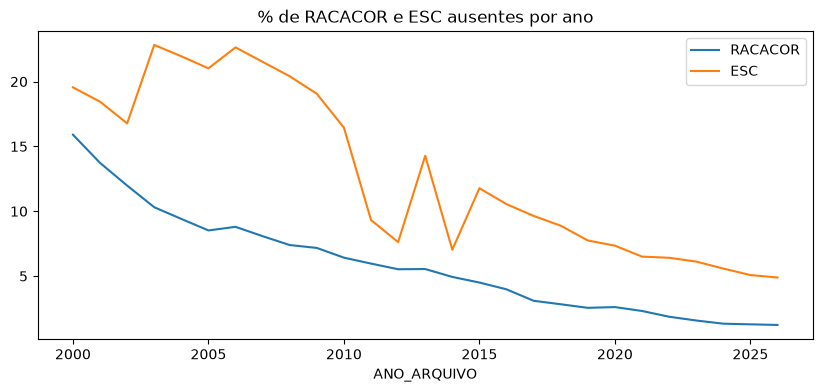
\includegraphics[width=0.95\textwidth]{figuras/ausentes_por_ano.png}
\caption{Percentual de registros com \texttt{RACACOR} e \texttt{ESC} ausentes,
  por ano (2000--2026). O código 9 (``ignorado''), que é um valor preenchido,
  não aparece nesta contagem e é tratado à parte.}
\label{fig:ausentes}
\end{figure}

\textbf{Preparação e estratégia de tratamento.} A preparação é feita por uma
única função, compartilhada por todos os notebooks, e seu resultado é
armazenado em cache (Parquet) cuja chave inclui o tamanho e a data de
modificação de cada CSV e uma constante de versão, de modo que um cache
desatualizado nunca é usado silenciosamente. As decisões foram:

\begin{itemize}
  \item \textbf{Idade:} decodificada para anos completos a partir do código do
    SIM (primeiro dígito indica a unidade --- minutos, horas, dias, meses,
    anos --- e os dois últimos, o valor).
  \item \textbf{Escolaridade e raça/cor:} mapeadas para categorias nomeadas,
    com \textbf{``Ignorado'' como categoria explícita} em vez de imputação.
    Nenhuma linha é descartada por esse motivo: ``Ignorado'' soma 26,409\%
    em \texttt{ESC} (8.616.946 registros) e 5,389\% em \texttt{RACACOR}
    (1.758.238). Descartar essas linhas enviesaria a amostra contra os anos
    iniciais da série. O código 0 de \texttt{ESC}, que aparece apenas em 2009
    a 2012 e em 2014 (231.933 registros, 0,711\%) e não consta do dicionário
    do SIM, foi mapeado para ``Ignorado''; essa é uma decisão discutível,
    isolada em uma única constante do código e revisável.
  \item \textbf{Município:} truncado para 6 dígitos e agregado em
    \textbf{unidade da federação}. O modelo nunca vê o município: são cerca de
    5.600 municípios distintos, o que inviabilizaria a codificação one-hot e,
    principalmente, aumentaria o risco de reidentificação em células pequenas
    (Seção~\ref{sec:etica}). As 27 UFs estão todas presentes, de São Paulo
    (23,196\% dos registros) a Roraima (0,175\%).
  \item \textbf{Filtros, com contabilidade.} Foram descartados 15.842
    registros com \texttt{SEXO} ignorado (0,0486\%), 81.308 com idade
    desconhecida (0,2492\%) e 3 cujo \texttt{CAUSABAS} não corresponde a
    nenhum capítulo da CID-10. O total descartado é de 97.153 registros
    (0,2977\% do bruto), restando \textbf{32.531.918 registros e 19 classes},
    sem nenhum valor nulo em nenhuma coluna.
\end{itemize}

\textbf{Distribuição do alvo.} A Tabela~\ref{tab:classes} e a
Figura~\ref{fig:distribuicao} mostram as 19 classes. O capítulo IX (doenças do
aparelho circulatório) concentra 27,0141\% dos registros, e o capítulo VII
(doenças do olho e anexos), 0,0019\% --- uma razão de 13.972 entre o maior e o
menor. Cinco capítulos ficam abaixo de 0,5\% dos registros. É esse quadro, e
não uma preferência genérica por ``robustez em dados tabulares'', que justifica
as escolhas metodológicas: com 19 classes e essa razão de desbalanceamento,
são necessários um baseline explícito, pesos balanceados e métricas
macro-agregadas para que o resultado signifique alguma coisa.

\begin{table}[ht]
\centering
\caption{Distribuição do alvo: capítulos da CID-10 observados em 32.531.918
  registros (SIM, Brasil, 2000--2026).}
\label{tab:classes}
\begin{tabular}{|l|l|r|r|}
\hline
\textbf{Cap.} & \textbf{Descrição} & \textbf{Registros} & \textbf{\%} \\
\hline
IX    & Doenças do aparelho circulatório                       & 8.788.199 & 27,0141 \\
II    & Neoplasias (tumores)                                   & 5.108.490 & 15,7030 \\
XX    & Causas externas de morbidade e mortalidade             & 3.712.335 & 11,4114 \\
X     & Doenças do aparelho respiratório                       & 3.516.512 & 10,8094 \\
XVIII & Sintomas, sinais e causas mal definidas                & 2.328.478 &  7,1575 \\
I     & Doenças infecciosas e parasitárias                     & 2.108.449 &  6,4812 \\
IV    & Doenças endócrinas, nutricionais e metabólicas         & 1.896.126 &  5,8285 \\
XI    & Doenças do aparelho digestivo                          & 1.614.124 &  4,9617 \\
XIV   & Doenças do aparelho geniturinário                      &   879.273 &  2,7028 \\
VI    & Doenças do sistema nervoso                             &   854.902 &  2,6279 \\
XVI   & Afecções originadas no período perinatal               &   632.965 &  1,9457 \\
V     & Transtornos mentais e comportamentais                  &   336.307 &  1,0338 \\
XVII  & Malformações congênitas e anomalias cromossômicas      &   271.194 &  0,8336 \\
III   & Doenças do sangue e transtornos imunitários            &   165.129 &  0,5076 \\
XII   & Doenças da pele e do tecido subcutâneo                 &   134.961 &  0,4149 \\
XIII  & Doenças do sistema osteomuscular e tecido conjuntivo   &   132.556 &  0,4075 \\
XV    & Gravidez, parto e puerpério                            &    46.798 &  0,1439 \\
VIII  & Doenças do ouvido e da apófise mastoide                &     4.491 &  0,0138 \\
VII   & Doenças do olho e anexos                               &       629 &  0,0019 \\
\hline
\end{tabular}
\end{table}

\begin{figure}[ht]
\centering
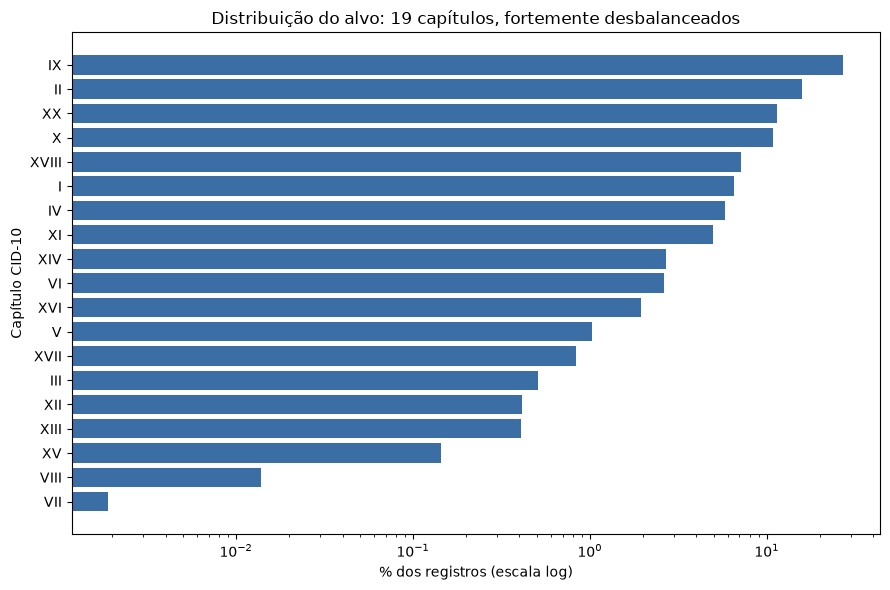
\includegraphics[width=0.85\textwidth]{figuras/distribuicao_capitulos.png}
\caption{Participação de cada capítulo da CID-10 no total de registros, em
  escala logarítmica. Os capítulos XIX e XXI não aparecem porque nunca ocorrem
  como causa básica nesta base.}
\label{fig:distribuicao}
\end{figure}

\section{Resultados Parciais}
\label{sec:resultados}

\subsection{Aspectos éticos e responsabilidade no uso da IA}
\label{sec:etica}

\textbf{Privacidade e LGPD.} O projeto usa exclusivamente os microdados
públicos do SIM, publicados como dados abertos pelo Ministério da Saúde sob
licença CC-BY, e os utiliza como foram disponibilizados. Das 8 colunas lidas,
nenhuma é identificador direto (nome, CPF, endereço). A Lei Geral de Proteção
de Dados Pessoais~\cite{lgpd} define dado anonimizado como aquele ``relativo a
titular que não possa ser identificado, considerando a utilização de meios
técnicos razoáveis e disponíveis na ocasião de seu tratamento'' (art.~5º,
inciso III) e estabelece, no art.~12, que dados anonimizados não são
considerados dados pessoais, \emph{salvo} quando a anonimização puder ser
revertida com esforços razoáveis. É exatamente essa ressalva que nos obriga a
cuidado: a combinação de quase-identificadores (idade, município de residência
e data do óbito) pode permitir reidentificação por inferência em municípios
pequenos ou para causas raras. As medidas concretas adotadas são:

\begin{itemize}
  \item \textbf{Uso restrito a dados públicos e anonimizados}, sem qualquer
    tentativa de reidentificação e sem cruzamento com outras bases.
  \item \textbf{Minimização de atributos.} Os modelos usam cinco variáveis, e
    a localização entra apenas no nível de UF: \texttt{CODMUNRES} é reduzido a
    município de 6 dígitos e daí a UF, e somente a UF é entrada do modelo. A
    data completa do óbito é lida na exploração, mas não entra no quadro de
    modelagem, que guarda apenas o ano do arquivo. Assim, nos modelos e nos
    resultados de classificação, nada é reportado abaixo do nível de UF.
  \item \textbf{Supressão de grupos pequenos.} O grupo adota a política de
    \textbf{suprimir de qualquer material publicado toda célula de resultado
    com menos de 10 casos} (por exemplo, cruzamentos UF $\times$ capítulo ou
    município $\times$ capítulo). Registre-se que essa é uma política adotada,
    \emph{ainda não implementada em código}. Na situação atual ela não é
    acionada pelos resultados de classificação: a menor classe (capítulo VII)
    tem 629 registros no total e 126 no conjunto de teste, e a menor UF
    (Roraima) tem 56.878 registros. As tabelas exploratórias dos notebooks são
    material de diagnóstico, não resultados publicados; nelas, as únicas
    contagens abaixo de 10 são o código 9 de \texttt{RACACOR}, que ocorre 5
    vezes em todo o período, e os 3 registros sem capítulo CID-10 --- em ambos
    os casos, contagens nacionais de uma única variável, sem cruzamento com
    município.
  \item \textbf{Tratamento dos arquivos.} Os CSVs brutos e o cache derivado não
    são versionados no repositório público; ficam versionados apenas o código,
    os resultados agregados e a documentação.
\end{itemize}

\textbf{Vazamento de rótulo como questão ética, e não apenas técnica.} Um
modelo que ``acertasse'' a causa porque leu a descrição da causa não mediria
associação nenhuma, e reportá-lo como resultado seria enganoso. A prevenção
estrutural e verificada em código descrita na Seção~\ref{sec:metodologia} é,
portanto, também uma exigência de honestidade na apresentação dos resultados.

\textbf{Viés de dados.} O não-preenchimento de \texttt{RACACOR} e \texttt{ESC}
é grande e muda muito ao longo dos anos (Figura~\ref{fig:ausentes}). Um modelo
treinado sobre esses dados herda qualquer padrão sistemático desse
não-preenchimento --- por exemplo, se a ausência for mais comum em certos
serviços de saúde ou regiões, algo que não medimos. Por isso mantemos
``Ignorado'' como categoria explícita em vez de imputar valores, o que
esconderia o viés em vez de expô-lo. Reconhecemos como limitação que ainda não
realizamos análise de erro por subgrupo (raça/cor, sexo, UF), prevista para a
etapa seguinte do projeto.

\textbf{Uso pretendido e mau uso.} O objetivo é apoiar o planejamento em saúde
pública em nível agregado. O modelo \textbf{não deve} ser usado para decisões
individuais sobre pessoas vivas, nem para inferir a causa de uma morte
específica sem o laudo médico, que é a fonte de verdade. O desempenho absoluto
medido (Seção~\ref{sec:desempenho}) reforça essa restrição: um F1-macro em
torno de 0,14 é incompatível com qualquer uso individual.

\textbf{Transparência.} O alvo é o capítulo da CID-10, e não o código
completo. Além de evitar centenas de classes, isso produz uma categoria ampla
e auditável, que reduz o risco de decisões automatizadas granulares e mal
calibradas a partir de poucas variáveis sociodemográficas. Todo o código,
incluindo a preparação e as asserções de ausência de vazamento, é público.

\textbf{Necessidade de submissão ao Comitê de Ética em Pesquisa (CEP).} O
projeto usa exclusivamente dados públicos, secundários e anonimizados, sem
acesso a registros identificáveis, sem vinculação com outras bases e sem
contato com pessoas. A Resolução CNS nº 510/2016~\cite{cns510}, em seu art.~1º,
parágrafo único, determina que não serão registradas nem avaliadas pelo sistema
CEP/CONEP, entre outras, a ``pesquisa que utilize informações de acesso
público, nos termos da Lei nº 12.527, de 18 de novembro de 2011'' (inciso II) e
a ``pesquisa que utilize informações de domínio público'' (inciso III).
Registre-se que essa resolução dispõe especificamente sobre pesquisas em
Ciências Humanas e Sociais, de modo que sua aplicação a este projeto é
analógica. Somando esse dispositivo à avaliação do professor orientador no
parecer da Parte 1, o grupo conclui que, em princípio, a submissão ao CEP
não é necessária. Isso mudaria se o projeto passasse a usar registros
identificáveis ou de acesso restrito, cruzasse o SIM com outra base ou
envolvesse contato direto com pessoas; nenhuma dessas condições se aplica
hoje, e, se alguma passar a valer, a necessidade de submissão deve ser
reavaliada antes de prosseguir.

\subsection{Detalhamento dos resultados parciais}
\label{sec:desempenho}

Os três modelos foram treinados sobre as 26.025.534 linhas de treino
\emph{completas}, sem subamostragem, e avaliados sobre as mesmas 6.506.384
linhas de teste, em um servidor Linux, com treino paralelizado em todos os
núcleos disponíveis (\texttt{n\_jobs = -1}). As configurações são iniciais e
nenhum hiperparâmetro foi ajustado: baseline de
classe majoritária; Random Forest com 100 árvores e profundidade máxima 12;
XGBoost com 100 rodadas, profundidade 6, taxa de aprendizado 0,3 e
\texttt{tree\_method = "hist"}. Os dois modelos receberam os mesmos pesos de
amostra balanceados.

\begin{table}[ht]
\centering
\caption{Comparação dos três modelos no conjunto de teste (6.506.384 linhas,
  divisão estratificada 80/20). A acurácia consta apenas como referência.}
\label{tab:comparacao}
\begin{tabular}{|l|r|r|r|r|}
\hline
\textbf{Modelo} & \textbf{F1-macro} & \textbf{Acurácia} & \textbf{Recall macro}
  & \textbf{Tempo de treino} \\
\hline
Baseline (classe majoritária) & 0,0224 & 0,2701 & 0,0526 &     3,1 s \\
Random Forest                 & 0,1329 & 0,1625 & 0,2234 &   343,9 s \\
XGBoost                       & \textbf{0,1406} & 0,1755 & 0,2294 &   983,3 s \\
\hline
\end{tabular}
\end{table}

\textbf{(a) Margem sobre o baseline.} Em F1-macro, o Random Forest supera o
baseline em $+0{,}1105$ (5,9 vezes) e o XGBoost em $+0{,}1183$ (6,3 vezes). Os
dois modelos também superam o baseline em recall macro (0,2234 e 0,2294 contra
0,0526). Em acurácia, porém, o baseline vence (0,2701 contra 0,1625 e 0,1755).
Esse resultado não é um defeito, e sim a consequência direta e prevista dos
pesos balanceados: o baseline atinge 27\% de acurácia prevendo sempre o
capítulo IX e errando todas as outras 18 classes, enquanto os modelos
ponderados distribuem suas predições entre as classes e abrem mão dos acertos
fáceis na classe majoritária. É precisamente por isso que a acurácia não é o
critério deste trabalho.

\textbf{(b) Desempenho por classe.} A Tabela~\ref{tab:recall} traz o recall
das 19 classes nos três modelos. O baseline tem recall 1,0 no capítulo IX e
\textbf{zero em 18 classes}; Random Forest e XGBoost não deixam nenhuma classe
com recall exatamente zero, embora no Random Forest os capítulos III (0,0004)
e IX (0,0013) tenham recall praticamente nulo. Apenas os capítulos XV
(gravidez, parto e puerpério) e XVI (perinatal) ultrapassam 0,5 de recall nos
dois modelos; o capítulo XX (causas externas) ultrapassa 0,5 somente no Random
Forest (0,5363 contra 0,4975 do XGBoost). Esse padrão confirma a expectativa
registrada na Seção~\ref{sec:metodologia}: idade e sexo quase determinam XV e
XVI, mas dizem pouco sobre as causas que competem entre si na população adulta
e idosa.

\begin{table}[ht]
\centering
\caption{Recall por classe nos três modelos, com o suporte de cada classe no
  conjunto de teste.}
\label{tab:recall}
\begin{tabular}{|l|l|r|r|r|r|}
\hline
\textbf{Cap.} & \textbf{Descrição} & \textbf{Suporte} & \textbf{Baseline}
  & \textbf{RF} & \textbf{XGBoost} \\
\hline
I     & Infecciosas       &   421.690 & 0,0000 & 0,0224 & 0,0281 \\
II    & Neoplasias        & 1.021.698 & 0,0000 & 0,1765 & 0,2473 \\
III   & Sangue/imunitário &    33.026 & 0,0000 & 0,0004 & 0,0058 \\
IV    & Endócrinas        &   379.225 & 0,0000 & 0,1546 & 0,1491 \\
V     & Mentais           &    67.261 & 0,0000 & 0,3006 & 0,3058 \\
VI    & Nervoso           &   170.980 & 0,0000 & 0,2794 & 0,2767 \\
VII   & Olho              &       126 & 0,0000 & 0,0794 & 0,0476 \\
VIII  & Ouvido            &       898 & 0,0000 & 0,0278 & 0,0768 \\
IX    & Circulatório      & 1.757.640 & 1,0000 & 0,0013 & 0,0260 \\
X     & Respiratório      &   703.302 & 0,0000 & 0,1099 & 0,1011 \\
XI    & Digestivo         &   322.825 & 0,0000 & 0,0763 & 0,0805 \\
XII   & Pele              &    26.992 & 0,0000 & 0,0987 & 0,1236 \\
XIII  & Osteomuscular     &    26.511 & 0,0000 & 0,0886 & 0,0454 \\
XIV   & Geniturinário     &   175.855 & 0,0000 & 0,0593 & 0,1022 \\
XV    & Gravidez/parto    &     9.360 & 0,0000 & 0,9701 & 0,9754 \\
XVI   & Perinatal         &   126.593 & 0,0000 & 0,8602 & 0,8373 \\
XVII  & Malformações      &    54.239 & 0,0000 & 0,2003 & 0,2404 \\
XVIII & Mal definidas     &   465.696 & 0,0000 & 0,2023 & 0,1924 \\
XX    & Causas externas   &   742.467 & 0,0000 & 0,5363 & 0,4975 \\
\hline
\end{tabular}
\end{table}

\textbf{(c) Leitura das matrizes de confusão.} As Figuras~\ref{fig:cmrf}
e~\ref{fig:cmxgb} mostram as matrizes normalizadas por linha, em que a diagonal
é o recall e cada linha soma 1 --- normalização necessária para que classes
raras sejam visíveis ao lado de um capítulo com 1,75 milhão de casos de teste.
Nos dois modelos a diagonal só se destaca em XV, XVI e XX. A confusão mais
sistemática ocorre entre XVII (malformações congênitas) e XVI (perinatal): no
Random Forest, 60\% dos casos de XVII são previstos como XVI, o que é
plausível, já que as duas causas se concentram nas primeiras idades e o modelo
só enxerga idade, sexo, raça/cor, escolaridade e UF. Fora desses blocos, as
predições se espalham amplamente, o que é a expressão visual do baixo
desempenho global.

\begin{figure}[ht]
\centering
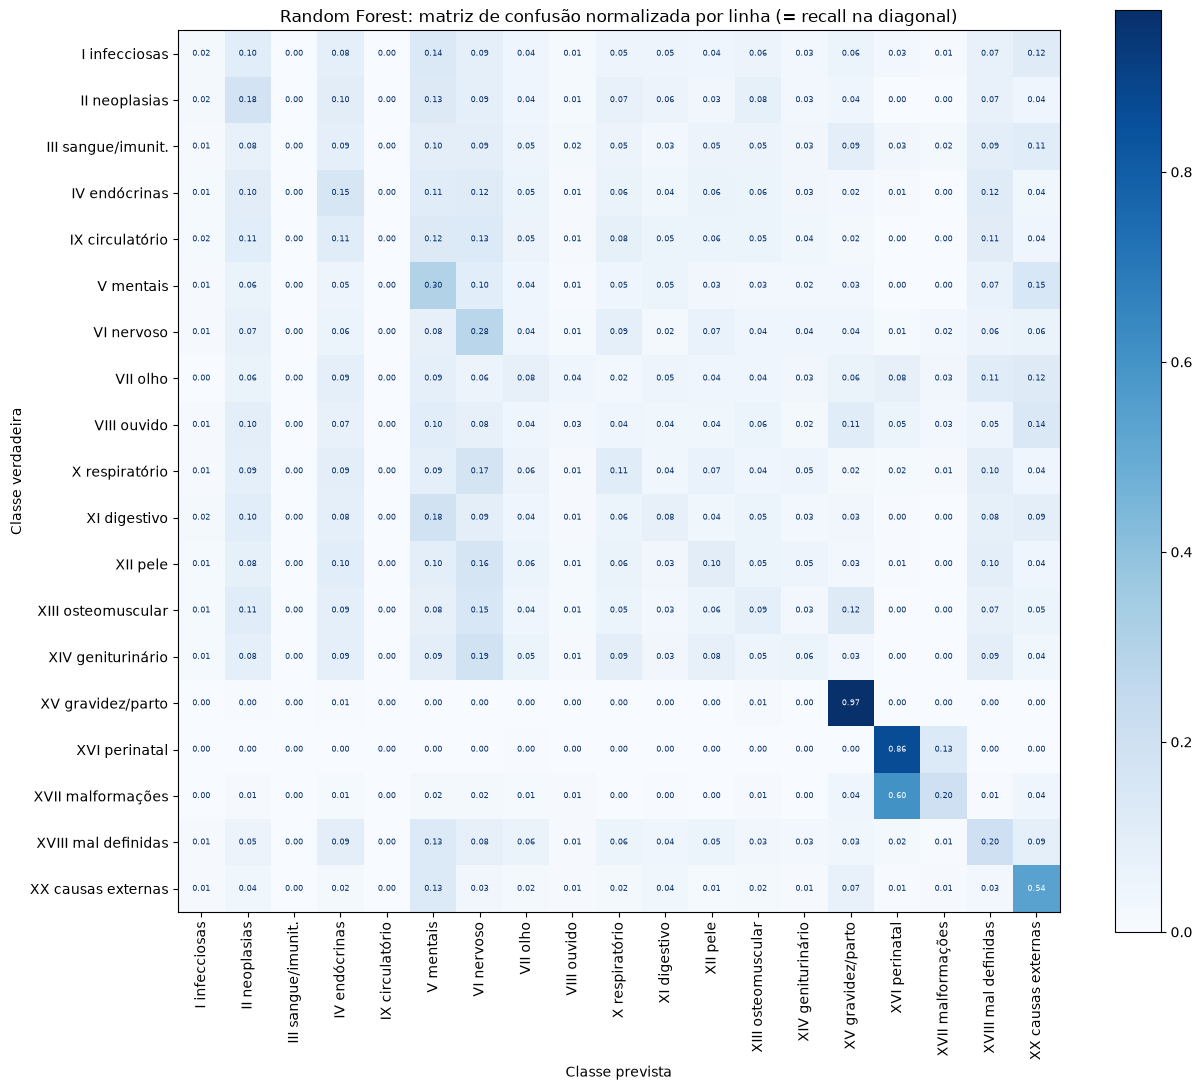
\includegraphics[width=\textwidth]{figuras/matriz_confusao_rf.png}
\caption{Random Forest: matriz de confusão normalizada por linha. A figura serve
  à leitura do padrão de confusão entre capítulos; os valores exatos da diagonal
  (o recall de cada classe) estão na Tabela~\ref{tab:recall}.}
\label{fig:cmrf}
\end{figure}

\begin{figure}[ht]
\centering
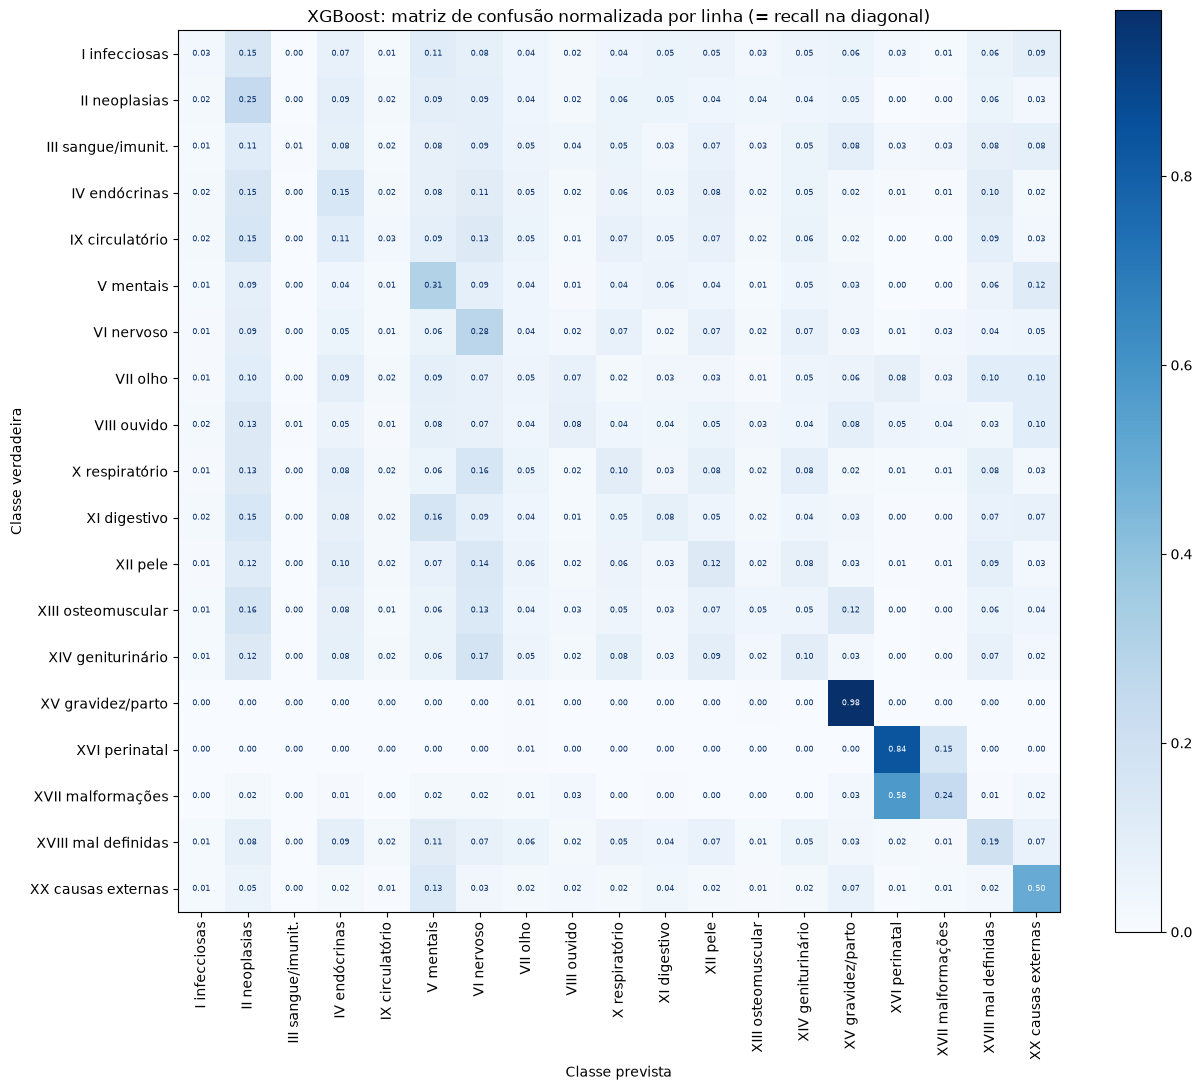
\includegraphics[width=\textwidth]{figuras/matriz_confusao_xgb.png}
\caption{XGBoost: matriz de confusão normalizada por linha. Como na
  Figura~\ref{fig:cmrf}, os valores exatos da diagonal estão na
  Tabela~\ref{tab:recall}.}
\label{fig:cmxgb}
\end{figure}

\textbf{(d) Classes raras.} Nos capítulos VII (olho) e VIII (ouvido), os
números são apenas indicativos. Em VII, com 126 casos de teste, o Random
Forest acerta 10 e o XGBoost 6, com precisão praticamente nula nos dois ---
consequência esperada do peso de amostra de 2.723 atribuído a essa classe, que
leva o modelo a prever VII para muitas linhas de outras classes. Em VIII, com
898 casos, o Random Forest acerta 25 e o XGBoost 69. O capítulo XV, apesar de
raro (9.360 casos), é o mais fácil de reconhecer (recall 0,9701 e 0,9754), mas
com precisão de apenas 0,039 nos dois modelos, porque muitas mulheres jovens
morrem de outras causas. Nenhum capítulo foi fundido ou removido.

\textbf{(e) XGBoost contra Random Forest: o ganho compensa o custo?} O XGBoost
obteve F1-macro 0,0078 maior (cerca de 6\% em termos relativos) gastando 983,3
s contra 343,9 s de treino, ou seja, 2,86 vezes mais tempo. Na checagem
temporal a razão foi ainda maior (1.322,3 s contra 352,9 s). O ganho aparece em
alguns capítulos (II: 0,2473 contra 0,1765; XIV: 0,1022 contra 0,0593; IX:
0,0260 contra 0,0013) e se inverte em outros (XVI: 0,8602 contra 0,8373; XX:
0,5363 contra 0,4975; XIII: 0,0886 contra 0,0454). Como as duas configurações
iniciais têm profundidades diferentes (12 e 6) e nenhuma foi ajustada, esta
comparação \emph{não} mostra qual família é superior após ajuste fino. Nossa
leitura, para o estágio atual: o Random Forest é a opção mais barata e chega
perto; o XGBoost passa a valer o custo se o ajuste de hiperparâmetros ampliar
a vantagem, o que ainda precisa ser verificado.

\textbf{(f) Checagem suplementar de generalização temporal.} Treinando com
2000--2022 (27.506.105 linhas) e testando em anos não vistos
(Tabela~\ref{tab:temporal}), o F1-macro cai de forma leve e monótona: 0,0051
do Random Forest e 0,0053 do XGBoost entre 2023 e 2026. O F1-macro agregado do
teste temporal fica cerca de 0,01 abaixo do protocolo principal. Essa
comparação, porém, \emph{não isola} a deriva temporal, porque o conjunto de
treino tem outro tamanho e o de teste é um conjunto diferente de anos, com
outra mistura de classes; o baseline não foi recalculado nessa checagem. A
mudança na qualidade do preenchimento ao longo dos anos é uma explicação
possível para a deriva, mas não foi testada. O ano de 2026 é parcial (506.027
linhas contra 1.463.485 em 2023), o que torna seu F1-macro menos estável.

\begin{table}[ht]
\centering
\caption{Checagem suplementar de generalização temporal: treino com 2000--2022,
  teste em anos não vistos. F1-macro.}
\label{tab:temporal}
\begin{tabular}{|l|r|r|r|r|}
\hline
\textbf{Modelo} & \textbf{2023} & \textbf{2025} & \textbf{2026 (parcial)}
  & \textbf{Agregado} \\
\hline
Random Forest & 0,1253 & 0,1216 & 0,1202 & 0,1230 \\
XGBoost       & 0,1340 & 0,1297 & 0,1287 & 0,1314 \\
\hline
\end{tabular}
\end{table}

\textbf{(g) Interpretação honesta do desempenho absoluto.} O resultado
principal é que \textbf{o desempenho absoluto é baixo}: um F1-macro de 0,13 a
0,14 significa que a maioria dos 19 capítulos é reconhecida de forma fraca. O
ganho sobre o baseline é real e grande em termos relativos, e mostra que os
modelos aprenderam algo --- mas o que eles aprenderam é, essencialmente, o
efeito de idade e sexo sobre um punhado de capítulos. Nossa interpretação é
que cinco atributos sociodemográficos carregam \emph{pouco} sinal sobre a
categoria da causa básica de óbito, o que é em si uma informação relevante: a
maior parte dos óbitos ocorre em adultos e idosos, faixa em que os capítulos
principais (circulatório, neoplasias, respiratório, endócrino) competem dentro
do mesmo perfil demográfico. Não apresentamos esses números como um
classificador utilizável, e sim como a medida de um limite.

\subsection{Limitações e próximos passos (N2)}

As limitações reconhecidas são: (i) uma única divisão e uma única semente, sem
intervalos de confiança; (ii) hiperparâmetros não ajustados, com profundidades
diferentes entre os dois modelos; (iii) conclusões sobre os capítulos VII e
VIII apoiadas em 126 e 898 casos de teste; (iv) ausência de análise de erro por
subgrupo; (v) a decisão de mapear o código 0 de \texttt{ESC} para ``Ignorado'',
que pode significar ``nenhuma escolaridade''; e (vi) a política de supressão de
células com menos de 10 casos ainda não implementada em código.

Para o segundo bimestre, os caminhos previstos são: ajuste de hiperparâmetros
dos dois modelos sob o mesmo protocolo; avaliação de atributos adicionais que
comprovadamente não vazem o rótulo (por exemplo, local de ocorrência e
assistência médica, mediante verificação explícita); inclusão de variáveis
temporais, como mês e ano do óbito; variáveis agregadas em nível de município
com granularidade suficiente para respeitar a supressão de grupos pequenos; e
análise de erro por subgrupo, para avaliar equidade. A expectativa, dado o que
foi medido aqui, é de ganhos moderados: o limite observado parece vir do
conjunto de atributos, não da escolha do algoritmo.

\subsection{Endereço do repositório no GitHub}

Todo o material do projeto está em um repositório \textbf{público}:
\url{https://github.com/araujoviana/projeto1-IA-2026}. Ele contém este artigo
(fontes LaTeX e PDF), a descrição do dataset e o procedimento para obtê-lo
(\texttt{data/README.md}, sem os microdados brutos, que são um download
público de grande porte), os três notebooks Python executados com seus
resultados (\texttt{notebooks/}), o módulo de funções com testes
automatizados (\texttt{src/} e \texttt{tests/}) e o histórico completo de
alterações no Git. Todos os arquivos-fonte abrem com um cabeçalho contendo a
identificação dos integrantes, a síntese do conteúdo do arquivo e o histórico
de alterações no formato ``data --- autor --- descrição''.

\bibliographystyle{sbc}
\bibliography{referencias}

\end{document}
